\chapter{Project Overview}
\setcounter{minitocdepth}{1}
\minitoc
\newpage
\setcounter{secnumdepth}{3}

\section{Introduction}
This chapter provides an overview of the project scope, including the host company, identified problems, proposed solutions, and project objectives. It also discusses the existing e-commerce platform, Shopify, and highlights the areas where Converty can improve to better compete in the market.

\section{Anchor Organisation}
This section introduces the startup, Converty, and its services.
\subsection{Converty}
Converty is an advanced platform for building and managing high-converting online stores. Converty provides powerful tools and advanced features that enable business owners and merchants to create effective online stores without the need for programming skills \cite{convertywebsite}.

\begin{figure}[H]
  \centering
  
\includegraphics[width=0.3\textwidth]{Images/convertyLogo.jpeg}
  \caption{Converty Logo}
  \label{fig:Converty Logo}
\end{figure}

Converty provides a comprehensive suite of services designed to support online store management, customer relationship management (CRM), marketing automation, and detailed reporting. The core mission of Converty is to revolutionize the e-commerce landscape for small and medium-sized enterprises (SMEs) by offering an all-in-one solution that streamlines business processes, reduces operational costs, and enhances overall efficiency.
\newline

\subsection{Services}
Converty offers a comprehensive range of services to help businesses succeed in the e-commerce industry. These services include:

\begin{itemize}
  \item Creating and customizing online shops: Converty provides a user-friendly platform that allows business owners to easily create and customize their online stores without the need for programming skills.
  \item Integration with analytics tools: Converty seamlessly integrates with various analytics tools, providing valuable insights into customer behavior, sales performance, and marketing effectiveness.
  \item Integration with delivery companies: Converty offers integration with popular delivery companies, streamlining the order fulfillment process and ensuring efficient shipping and delivery.
  \item Order management: Converty provides robust order management features, allowing businesses to efficiently process and track orders, manage inventory, and handle returns and refunds.
  \item Product management: Converty's platform enables businesses to easily manage their product catalog, including adding new products, updating product information, and organizing products into categories.
  \item Customer relationship management (CRM): Converty's CRM features help businesses build and maintain strong relationships with their customers, including managing customer profiles, tracking customer interactions, and implementing targeted marketing campaigns.
  \item Marketing automation: Converty offers powerful marketing automation tools, allowing businesses to automate various marketing activities such as email campaigns, social media promotions, and personalized recommendations.
\end{itemize}

\section{Study Of The Existing}
Shopify is a complete commerce platform that lets anyone start, manage, and grow a business. You can use Shopify to build an online store, manage sales, market to customers, and accept payments in digital and physical locations. Shopify’s reputation as a commerce leader comes from listening to the experiences of millions of business owners. By supporting solopreneurs and enterprise brands, Shopify has built the features and products that power today’s businesses and will shape the future of commerce \cite{shopifyblog}.

Shopify is a popular e-Commerce platform that allows individuals and businesses to create online stores effortlessly. Among its many advantages are the performant templates that ensure fast loading times and a seamless shopping experience for customers.

In addition to high-performing templates, Shopify offers a variety of sales-boosting features. These include abandoned cart recovery, targeted email campaigns, and advanced analytics. These tools help store owners optimize their online sales and increase revenue.

Furthermore, Shopify provides a comprehensive mobile app that allows store owners to manage their business on the go. The app includes features like order management, product updates, and sales tracking, making it convenient to maintain an online store anytime, anywhere.

While Shopify is a well-established platform with a wide range of features, Converty aims to address some of the limitations and challenges faced by Shopify users. Converty focuses on providing a more streamlined and customizable experience, eliminating the need for multiple applications and reducing the complexity associated with extensive feature sets. By integrating essential tools directly into the platform, Converty offers a more efficient and user-friendly solution for managing online stores. This approach not only simplifies the user experience but also enhances performance and scalability, making it a strong competitor in the e-commerce market.

This comparison highlights the areas where Converty can improve to better compete with Shopify.

\section{Problem Statement} 
Despite Converty's notable progress in the e-commerce industry, the product, which consists of a web dashboard and a mobile application, currently faces several critical challenges that must be addressed to compete effectively with Shopify. These challenges include:

\begin{itemize} 
    \item \textbf{Performance Issues:} One of the four templates provided by Converty has performance problems that negatively affect the overall user experience. 
    \item \textbf{Missing Key Features:} The platform lacks essential features such as upselling, which are critical to maximizing sales and improving customer satisfaction. 
    \item \textbf{Incomplete Mobile App Experience:} The mobile app experience is incomplete, limiting accessibility and convenience for users who prefer to manage their online stores on mobile devices. 
\end{itemize} 

Addressing these challenges is crucial for Converty to fully leverage its potential and offer a robust, competitive solution in the e-commerce market. By enhancing performance, adding key features, and completing the mobile app experience, Converty can provide a more comprehensive and user-friendly platform that meets the needs of online store owners and merchants.

\section{Proposed Solution}
After a long discussion with the company, the following fixes were decided to be made:

\begin{itemize}
  \item \textbf{Performance Optimization:} The first template will be recoded using React to enhance performance. This will involve refactoring the codebase to improve efficiency and responsiveness, leading to a significantly better user experience.
  \item \textbf{Upsell Feature Integration:} An upsell feature will be added to the platform, incorporating algorithms and interfaces that recommend complementary products to customers. This feature aims to increase the average order value and boost customer satisfaction.
  \item \textbf{Mobile App Enhancements:} Key mobile features will be incorporated to complete the mobile app experience, ensuring a seamless and intuitive user interface for managing online stores on mobile devices.
\end{itemize}

These solutions are expected to significantly enhance Converty's platform, making it more competitive in the e-commerce market. By improving performance, adding key features, and completing the mobile app experience, Converty aims to provide a comprehensive and user-friendly solution for online store owners and merchants. These enhancements will help Converty attract new users, retain existing customers, and establish itself as a leading platform in the e-commerce industry.
\newline

\section{About the Project}
This section provides a comprehensive overview of the project, including its goals, objectives, deliverables, management plan, and timeline. It also discusses the Software Development Life Cycle (SDLC) model used for the project.

\subsection{Goals}
The primary goals of this project are to improve the performance of the Converty platform, introduce key features to enhance functionality, and complete the mobile app experience to ensure a seamless user interface across all devices.

\subsection{Objectives}
To achieve these goals, the following objectives were set:
\begin{itemize}
    \item Recode the first template using a new technology \textbf{React} to enhance performance.
    \item Integrate an upsell feature to boost average order value and customer satisfaction.
    \item Enhance the mobile app with essential features to provide a comprehensive and user-friendly experience.
\end{itemize}

\subsection{Deliverables}
The project deliverables include the following components:
\begin{itemize}
    \item \textbf{Source Code:} The complete source code, including all necessary files for building and running the project. The code should be well organized, adhere to the coding standards, and include comments for clarity.
    \item \textbf{Documentation:} Comprehensive documentation covering the project architecture, major modules, functions, and classes. It should also include setup instructions, usage examples, and relevant information for users and developers.
    \item \textbf{Presentation:} A presentation outlining the project's objectives, design, implementation, key features, challenges, and solutions. It should include visual aids such as diagrams, charts, and screenshots.
\end{itemize}

\subsection{Management Plan}
The management plan for this project follows the Agile SDLC model, which emphasizes iterative development, collaboration, and flexibility. The project is divided into several sprints, each focusing on specific tasks and deliverables.
To begin, let's look into the Software Development Life Cycle (SDLC) models.

\subsubsection{Software Development Life Cycle (SDLC)}
The SDLC employed for this project involved iterative development and continuous feedback to meet all project requirements effectively. Figure \ref{fig:SDLC Phases} illustrates the SDLC phases used in this project \cite{sdlc}.

\begin{figure}[H]
  \centering
  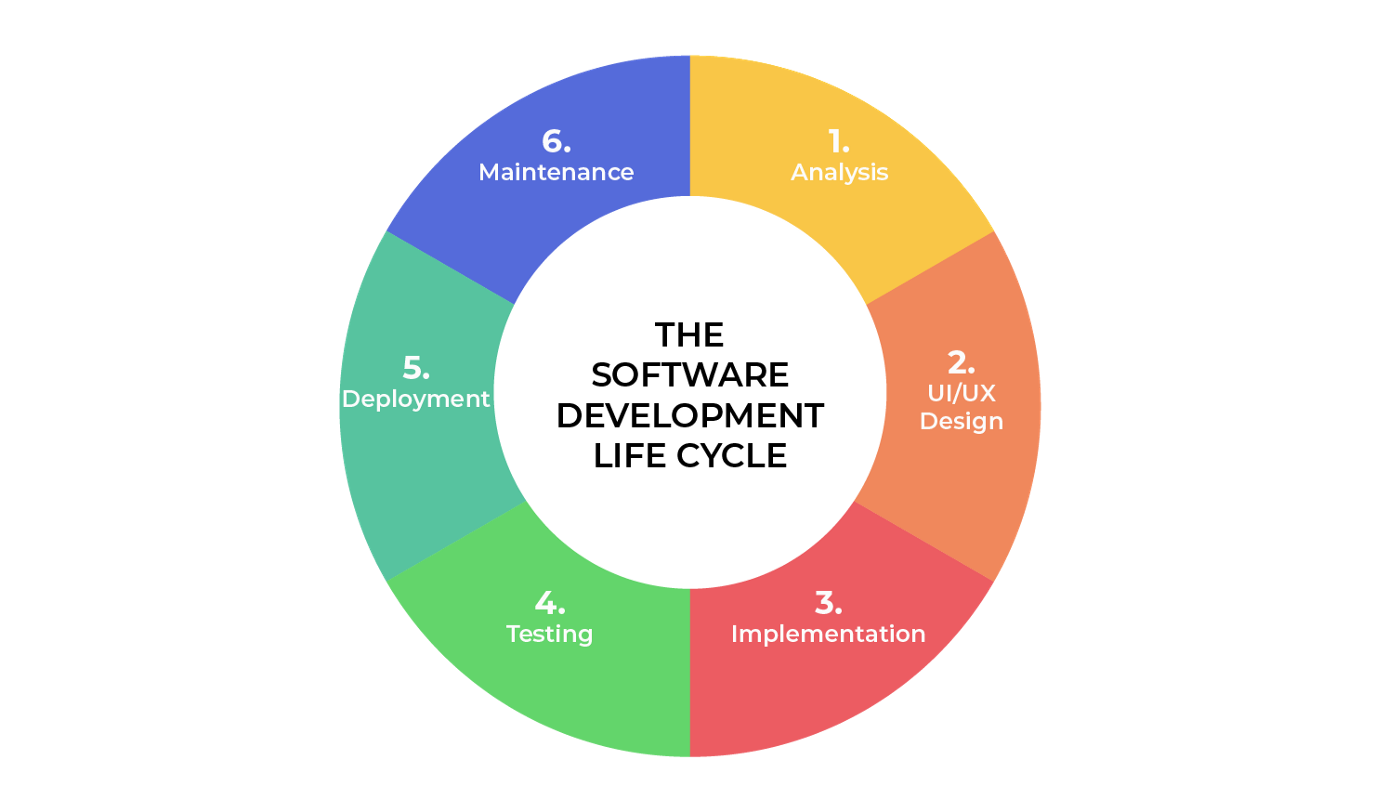
\includegraphics[width=0.8\textwidth]{Images/sdlc.png}
  \caption{SDLC Phases}
  \label{fig:SDLC Phases}
\end{figure}

\subsubsection{Comparison of SDLC Models}
To determine the most suitable SDLC model for this project, a comparison of different models was conducted. Table \ref{tab:sdlc_models} provides a comparison of the Waterfall, Agile, Scrum, and Kanban models, highlighting their advantages, disadvantages, and suitability.

\begin{longtable}{|m{3cm}|m{4cm}|m{4cm}|m{4cm}|}
\hline
\textbf{Model} & \textbf{Advantages} & \textbf{Disadvantages} & \textbf{Suitability} \\
\hline
\endfirsthead
\hline
\textbf{Model} & \textbf{Advantages} & \textbf{Disadvantages} & \textbf{Suitability} \\
\hline
\endhead
Waterfall Model & Simple and easy to understand and use & Inflexible, difficult to make changes once the process is underway & Suitable for small projects with well-defined requirements \\
\hline
Agile Model & Flexible and adaptive to changes, promotes collaboration and customer feedback & Can be difficult to predict effort required and can lead to scope creep & Suitable for projects with dynamic requirements \\
\hline
Scrum Model & Iterative approach promotes continuous improvement, increases team accountability & Requires experienced team members, can be difficult to implement for complex projects & Suitable for complex projects requiring frequent changes \\
\hline
Kanban Model & Visual workflow management, promotes continuous delivery & Lack of time frames can lead to lack of urgency & Suitable for projects needing continuous delivery and improvement \\
\hline
\caption{Comparison of SDLC Models}
\label{tab:sdlc_models}
\end{longtable}

\subsubsection{Agile Methodology}
After comparing various SDLC models, the Agile methodology was chosen for this project due to its flexibility, collaboration, customer feedback, and rapid releases. Agile supports adaptive planning and continuous improvement, making it ideal for dynamic and complex projects. Agile encourages iterative development cycles (sprints) that allow teams to adapt quickly to changing requirements and deliver functional software incrementally.

\subsubsection{Scrum Framework}
Within the Agile methodology, the Scrum framework was selected to manage the project's development process. Scrum, a subset of Agile, manages complex product development through iterative cycles known as sprints, which typically last 2-4 weeks. Key roles in Scrum include the Product Owner (responsible for project vision and backlog prioritization), the Scrum Master (facilitates the process and resolves issues), and the Development Team (completes the work). Scrum ceremonies such as sprint planning, daily stand-ups, sprint reviews, and retrospectives ensure ongoing progress and improvement. Figure \ref{fig:Scrum Framework} illustrates the Scrum framework used in this project \cite{scrumframework}.

\begin{figure}[H]
  \centering
  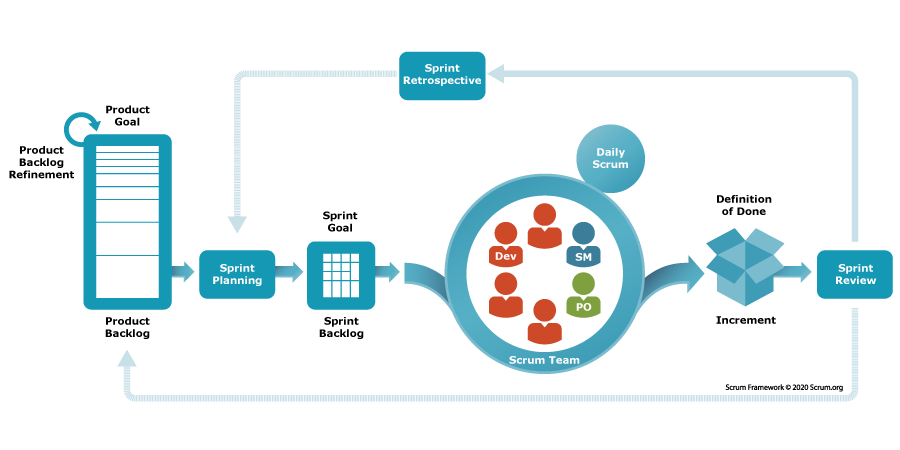
\includegraphics[width=1\textwidth]{Images/scrum.png}
  \caption{Scrum Framework}
  \label{fig:Scrum Framework}
\end{figure}

\subsubsection{Scrum Tools}
To support the Scrum framework, the following tools were utilized:
\begin{itemize}
    \item \textbf{GitHub:} For version control and collaborative code management, allowing team members to work on code simultaneously, track changes, and manage issues.
    \item \textbf{Google Meet:} For virtual meetings including daily stand-ups, sprint planning, reviews, and retrospectives, ensuring remote team members can collaborate effectively.
    \item \textbf{Notion:} An all-in-one workspace for project management, documentation, and collaboration, helping organize tasks, track progress, and maintain a shared knowledge base.
\end{itemize}

\subsection{Project Timeline}
The project timeline is outlined in Table \ref{tab:project_timeline}, which details the duration and key milestones for each sprint.

\begin{table}[h]
  \centering
  \begin{tabular}{|c|c|c|}
    \hline
    \textbf{Sprint} & \textbf{Duration} & \textbf{Key Milestones} \\
    \hline
    Sprint 1 & 4 weeks & Recreate the simple template \\
    \hline
    Sprint 2 & 4 weeks & Implement the upsell feature \\
    \hline
    Sprint 3 & 4 weeks & Enhance the mobile app with order management \\
    \hline
    Sprint 4 & 4 weeks & Add budget and costs management to the mobile app \\
    \hline
    Sprint 5 & 4 weeks & Integrate statistics management into the mobile app \\
    \hline
    Sprint 6 & 4 weeks & Develop the notifications center for the mobile app \\
    \hline
  \end{tabular}
  \caption{Project Timeline}
  \label{tab:project_timeline}
\end{table}

\subsubsection{Scrum Team}
The Scrum team for this project includes the following key roles:
\begin{itemize}
    \item \textbf{Product Owner:} Mr. Ayoub Nejem (CEO)
    \item \textbf{Scrum Master:} Mr. Sami Kammoun (Co-Founder and CTO)
\end{itemize}

\subsubsection{Product Backlog}
The product backlog contains all the tasks and user stories that need to be completed during the project. Table \ref{tab:product_backlog} outlines the product backlog, including the sprint, theme, user story ID, user story description, and priority.

\begin{longtable}{|c|p{6cm}|c|p{6cm}|c|}
\hline
\textbf{Sprint} & \textbf{Theme} & \textbf{ID} & \textbf{User Story} & \textbf{Priority} \\ 
\hline
\endfirsthead

\hline
\textbf{Sprint} & \textbf{Theme} & \textbf{ID} & \textbf{User Story} & \textbf{Priority} \\ 
\hline
\endhead

\hline
\endfoot

\hline
\endlastfoot

\multirow{1}{*}{1} & \multirow{1}{*}{Shop Visiting} & 1.1 & As a shop visitor, I want to access the shop landing page & High \\ \cline{3-5}
& & 1.2 & As a shop visitor, I want to load additional products & High \\ \cline{3-5}
& & 1.3 & As a shop visitor, I want to follow social media links & Medium \\ \cline{3-5}
& & 1.4 & As a shop visitor, I want to reach out to the support team & Medium \\ \cline{3-5}
& & 1.5 & As a shop visitor, I want to search for specific products & High \\ \cline{3-5}
& & 1.6 & As a shop visitor, I want to complete the checkout form & High \\ \cline{3-5}
& & 1.7 & As a shop visitor, I want to add items to the cart & High \\ \cline{3-5}
& & 1.8 & As a shop visitor, I want to purchase items & High \\ \cline{3-5}
& & 1.9 & As a shop visitor, I want to accept or decline offers & Medium \\ \hline
\multirow{1}{*}{2} & \multirow{1}{*}{Upsell Management} & 2.1 & As a shop admin, I want to display all upsells and cross-sells & High \\ \cline{3-5}
& & 2.2 & As a shop admin, I want to perform search operations & High \\ \cline{3-5}
& & 2.3 & As a shop admin, I want to edit upsell and cross-sell details & High \\ \cline{3-5}
& & 2.4 & As a shop admin, I want to delete upsell and cross-sell entries & Medium \\ \cline{3-5}
& & 2.5 & As a shop admin, I want to view previews & Medium \\ \hline
\multirow{1}{*}{3} & \multirow{1}{*}{Order Management} & 3.1 & As a shop admin, I want to display all orders & High \\ \cline{3-5}
& & 3.2 & As a shop admin, I want to view order details & High \\ \cline{3-5}
& & 3.3 & As a shop admin, I want to add or edit orders & High \\ \cline{3-5}
& & 3.4 & As a shop admin, I want to filter orders by status, product, or delivery company & Medium \\ \cline{3-5}
& & 3.5 & As a shop admin, I want to perform search operations & High \\ \hline
\multirow{1}{*}{4} & \multirow{1}{*}{Financial Management} & 4.1 & As a shop admin, I want to enter various cost parameters & High \\ \cline{3-5}
& & 4.2 & As a shop admin, I want to calculate key financial metrics & High \\ \cline{3-5}
& & 4.3 & As a shop admin, I want to view all budgets & High \\ \cline{3-5}
& & 4.4 & As a shop admin, I want to select specific budgets & Medium \\ \cline{3-5}
& & 4.5 & As a shop admin, I want to edit budget information & Medium \\ \cline{3-5}
& & 4.6 & As a shop admin, I want to view total balance, revenue, and expenses & High \\ \hline
\multirow{1}{*}{5} & \multirow{1}{*}{Statistical Analysis} & 5.1 & As a shop admin, I want to view different types of statistics & High \\ \cline{3-5}
& & 5.2 & As a shop admin, I want to filter statistical data & Medium \\ \hline
\multirow{1}{*}{6} & \multirow{1}{*}{Notification Center} & 6.1 & As a shop admin, I want to customize notification sounds & Medium \\ \cline{3-5}
& & 6.2 & As a shop admin, I want to receive real-time notifications & High \\ \hline

\caption{Product Backlog}
\label{tab:product_backlog}
\end{longtable}

\subsubsection{Gantt Chart}
A Gantt chart visually represents the project schedule, showing the start and end dates of various project elements, and helps track the project's timeline and progress. Figure \ref{fig:Gantt Chart} illustrates the Gantt chart for this project \cite{ganttchart}.

\begin{figure}[H]
  \centering
  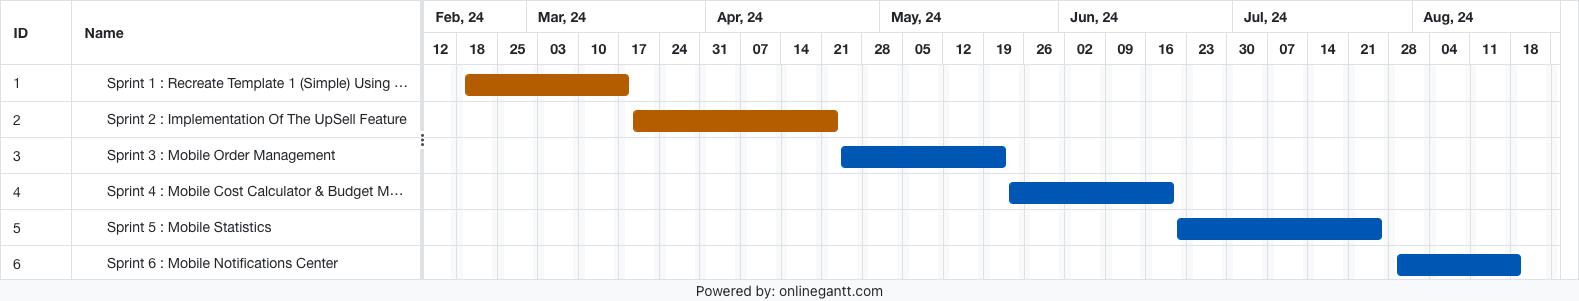
\includegraphics[width=1\textwidth]{Images/Online Gantt 20240715.png}
  \caption{Gantt Chart}
  \label{fig:Gantt Chart}
\end{figure}

\subsection{Conclusion}
In summary, this chapter outlined the scope of the project, detailing the host company, identified problems, and proposed solutions. The project aimed to optimize Converty's platform performance, add crucial features, and enhance the mobile app experience. The detailed management plan and timeline were presented to ensure effective project execution. By addressing the identified issues, the project aims to significantly improve Converty's functionality and user experience.